\documentclass[11pt]{article}
\usepackage{graphicx} 
\usepackage{listings}
\usepackage{comment} 

\title{
\begin{center}
\begin{Large}
{
\bf  \underline{Introduction to Data Science}
\bf

\bf  \underline{Text Classification}
}
\end{Large}\\[0.1 cm]
\begin{Large}
{\large {\bf Course Code: SWE 336}}\\[1 cm]
\end{Large}
{\large {\bf Submitted To,}}\\
{\large Ms Sayma Sultana Chowdhury}\\
{\large Assistant Professor}\\
{\large IICT, SUST}\\[1 cm]

{\large {\bf Submitted By,}}\\
{\large Gourab Saha}\\
{\large Reg: 2017831004}\\
{\large Session: 2017-18}\\
{\large SWE, IICT, SUST}\\
\end{center}
}

\begin{document}

\begin{figure}
\centering

\includegraphics[scale=.5]{sust}
\label{fig:Shahjalal University of Science and Technology}
\end{figure}

\maketitle
\newpage




\begin{center}
\bf  \underline{Assignment}
\end{center}


\section*{Problem:}

\begin{enumerate}
\bf{
\item{ Train five separate ML Classification models on this data and provide the classification report for each. Models: KNN, Naive Bayes, Random Forest, Decision Tree and ANN.}


\item{Why does it happen that the model gives very low f1 score for some classes but not the same for others?}


\item{Can you fix the low f1 score issue?}
}
\end{enumerate}
 
\section*{Answer:}

\begin{center}
\bf  \underline{Answer to Question No: 1} \\
\end{center} 


\section{Naive Bayes}
Naïve Bayes Classifier is one of the simple and most effective Classification algorithms which helps in building the fast machine learning models that can make quick predictions.
\begin{center}
\bf The accuracy, macro average and weighted average are given below(Naive Bayes Model).
\end{center}



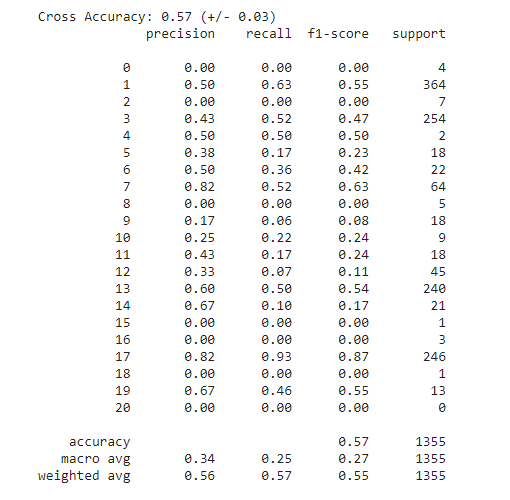
\includegraphics[width=11cm, height=7cm]{NaiveBayesModel}

\begin{center}
\bf Naive Bayes Model's Confusion Matrix.
\end{center}

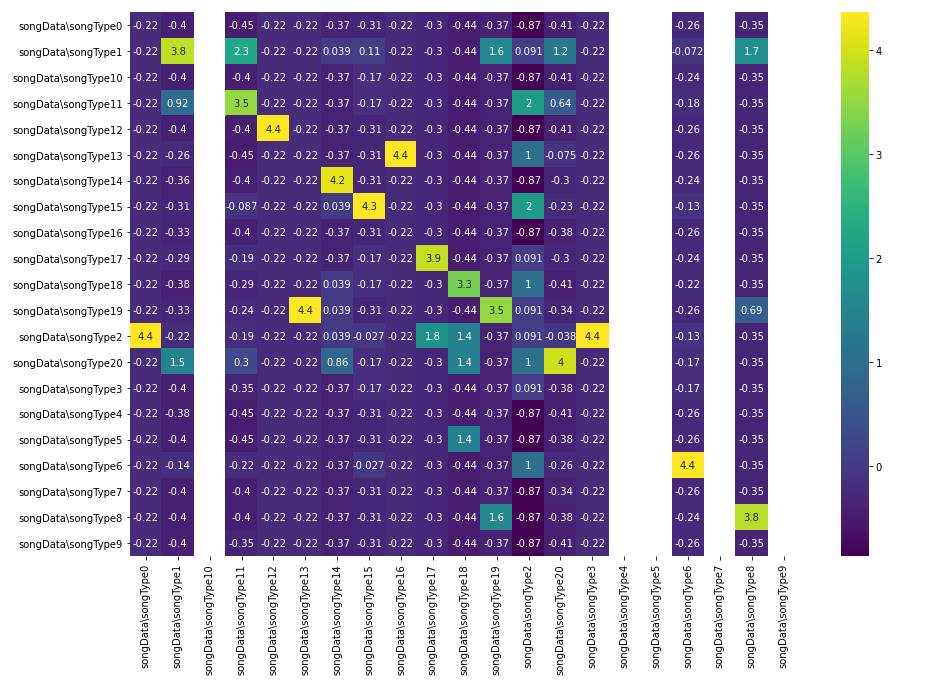
\includegraphics[scale=.6]{NaiveBayesMatrix}


\section{KNN}
K-Nearest Neighbors (KNN) is one of the simplest algorithms used in Machine Learning for regression and classification problem. KNN algorithms use data and classify new data points based on similarity measures (e.g. distance function). Classification is done by a majority vote to its neighbors.

\begin{center}
\bf The accuracy, macro average and weighted average are given below(KNN Model).
\end{center}

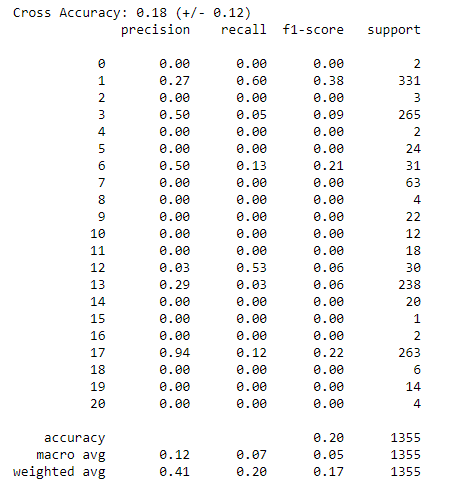
\includegraphics[width=11cm, height=7cm]{KNNModel}

\begin{center}
\bf KNN Model's Confusion Matrix.
\end{center}

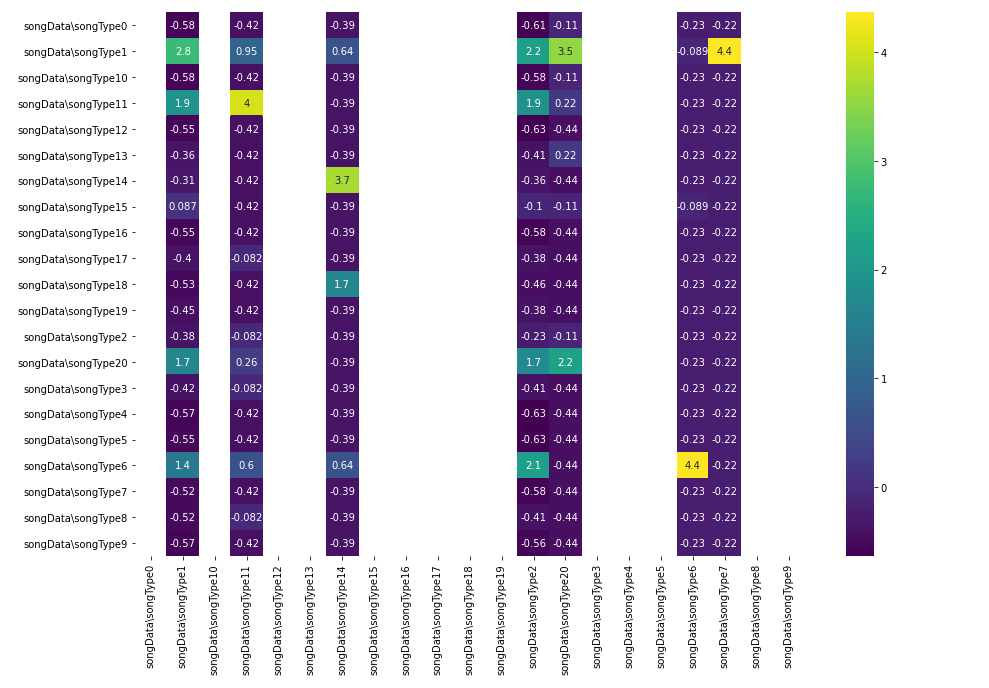
\includegraphics[scale=.6]{KNNMatrix}

\section{Decision Tree}
Decision Trees are a non-parametric supervised learning method used for both classification and regression tasks. Tree models where the target variable can take a discrete set of values are called classification trees.

\begin{center}
\bf The accuracy, macro average and weighted average are given below(Decision Tree Model).
\end{center}

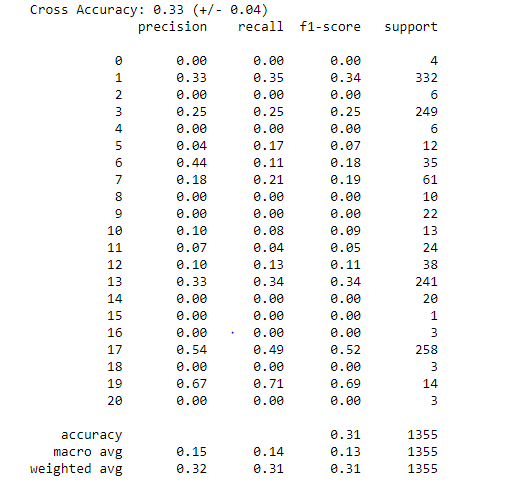
\includegraphics[width=11cm, height=7cm]{DecisionTreeModel}

\begin{center}
\bf Decision Tree Model's Confusion Matrix.
\end{center}

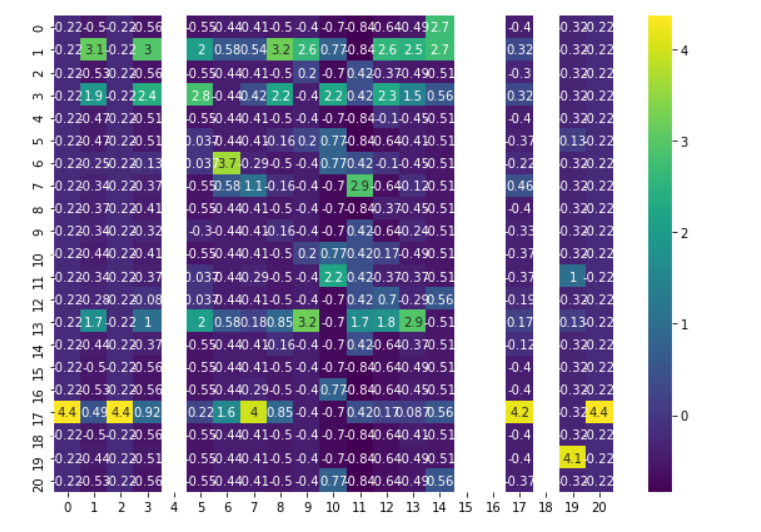
\includegraphics[width=16cm, height=7cm]{DecisionTreeMatrix}


\section{Random Forest}
Random forest is a flexible, easy to use machine learning algorithm that produces, even without hyper-parameter tuning, a great result most of the time. It is also one of the most used algorithms, because of its simplicity and diversity (it can be used for both classification and regression tasks).

\begin{center}
\bf The accuracy, macro average and weighted average are given below(Random Forest Model).
\end{center}

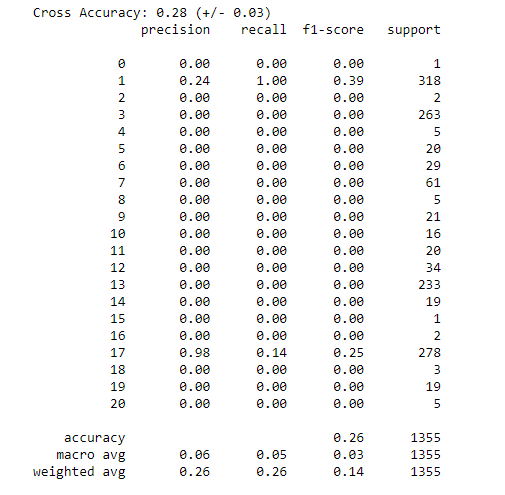
\includegraphics[width=11cm, height=6cm]{RandomForestModel}

\begin{center}
\bf Random Forest Model's Confusion Matrix.
\end{center}

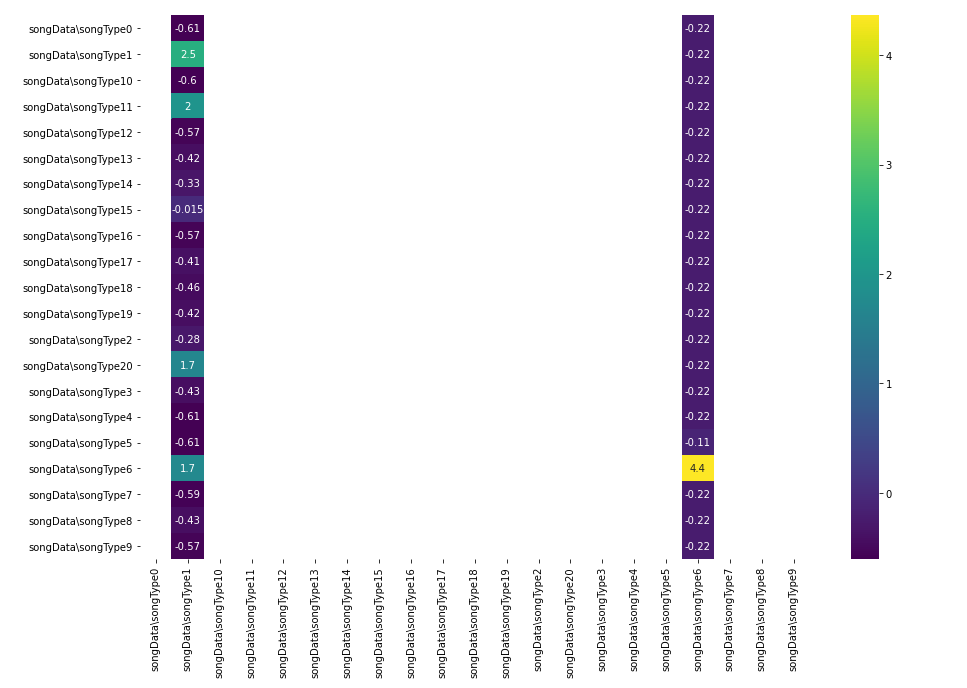
\includegraphics[width=16cm, height=7cm]{RandomForestMatrix}


\section{Artificial Neural Network}
An artificial neural network (ANN) is the piece of a computing system designed to simulate the way the human brain analyzes and processes information. It is the foundation of artificial intelligence (AI) and solves problems that would prove impossible or difficult by human or statistical standards.

\begin{center}
\bf The accuracy, macro average and weighted average are given below(Artificial Neural Network).
\end{center}

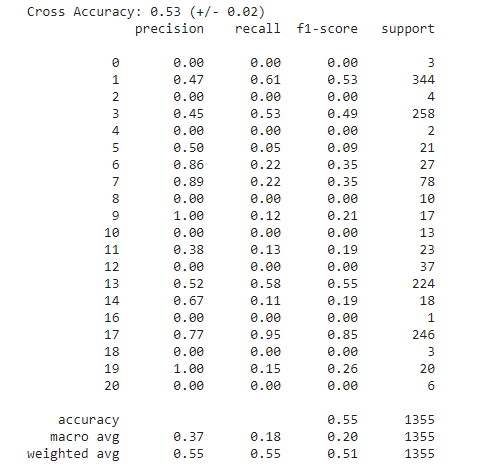
\includegraphics[width=11cm, height=7cm]{ArtificialNeuralNetworkModel}

\begin{center}
\bf Artificial Neural Network's Confusion Matrix.
\end{center}

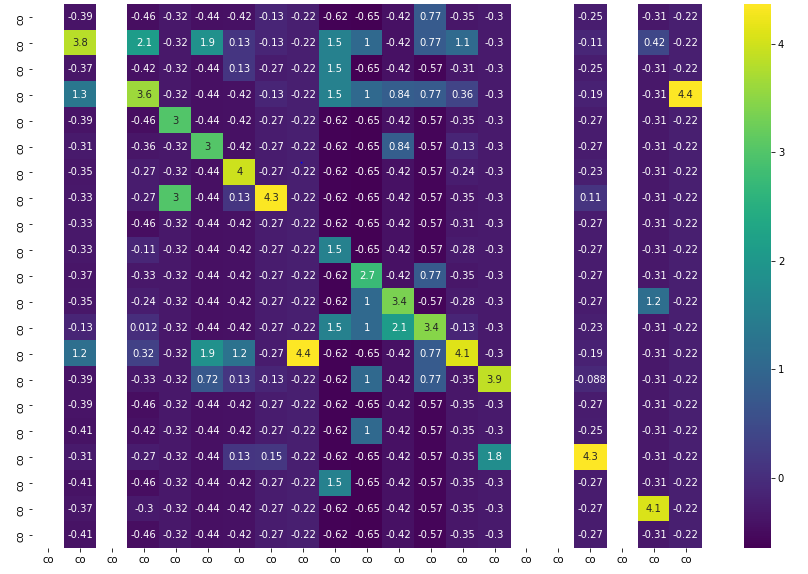
\includegraphics[width=16cm, height=6cm]{ArtificialNeuralNetworkMatrix}


\begin{center}
\bf  \underline{Answer to Question No: 2} \\ 
\end{center} 

The equation for calculating F1 score is:

\[
2*\frac{precision*recall}{precision + recall}
\]

So F1 is high when precision and recall both are high.If precision or
recall is low then F1 score will be low. Now, we know precision:

\[
\frac{True Positive}{True Positive + False Positive}
\]

The precision value will be high if False positive is low and precision will be low if False
positive is high and vice versa. If False positive is low for a specific song type that means
the model doesn’t say other type to be this type. So model perfectly predict this song
type. \\


If False positive is high for a specific class or category then model prediction is not
good for this category. It says other category to be this category. Recall:


\[
\frac{True Positive}{True Positive + False Negative}
\]


Recall will be high when False negative is low and recall will be low when False
negative is high. False negative low means most of the time model can predict correctly
a specific category. And few times it says a specific category to other category. If False
negative is high then model can’t predict a specific category correctly.
\\ 
So, F1 score is high when False positive and False negative bot is low.

\newpage
\begin{center}
\bf  \underline{Answer to Question No: 3} \\
\end{center} 

If the F1-score is the figure of merit, I would try to tune the class weights. It should be pretty
easy, if we have a binary classification problem. We can feed the class weight a dictionary with
the weights for each class. Here’s a little example.
\\
      

$clf = RandomForestClassifier()$ 

params = \{'class weight': [ \{0:neg weight, 1:1\} for neg weight in np.arange(1.0, 5.0, 0.5)]\}


gs = GridSearchCV(estimator= clf, param grid = params, cv = 5)

gs.fit X train, y train




\end{document}